\section{Use Graphics and Tables in \LaTeX}
\begin{frame}
	\tableofcontents[currentsection,hideothersubsections]
\end{frame}

\subsection{Measuring units}

\begin{frame}
	\frametitle{Measuring units in \LaTeX}
\end{frame}

\subsection{Include graphs}

\begin{frame}
	\frametitle{Include graphs}
	It's very useful to include graphs in \LaTeX, especially in report and paper writing. Here is a common template of including a single floating graph.
	\begin{command}
		\samplecommand{usepackage}\{graphicx\}\\
		\samplebegin{figure}[\structure{position}]\\
		\qquad\samplecommand{centering}\\
		\qquad\samplecommand{includegraphics}[\structure{options}]\{\structure{file}\}\\
		\qquad\samplecommand{caption}\{\structure{caption}\}\\
		\qquad\samplecommand{label}\{\structure{label}\}\\
		\sampleend{figure}
		\begin{itemize}
			\item \structure{position} - we usually use \structure{htbp} here
			\item \structure{options} - the width, height and other options about the graph
			\item \structure{caption} - the caption displayed above/under the graph
			\item \structure{label} - used for references in a document (will be introduced later)
		\end{itemize}
	\end{command}
\end{frame}

\begin{frame}
	Usually you need to optimize the size and some other properties of the graph, most of them can be set in \structure{options}. (Only some useful options are listed here)
	\begin{itemize}
		\item \structure{height} - use any \LaTeX\ measuring unit.
		\item \structure{width} - use any \LaTeX\ measuring unit.
		\item \structure{scale} - scale the graph to this proportion
		\item \structure{angle} - rotate the graph in anti-clockwise by this angle 
	\end{itemize}
	\begin{minipage}{0.45\linewidth}
		\begin{example}
			\begin{figure}[htbp]
				\centering
				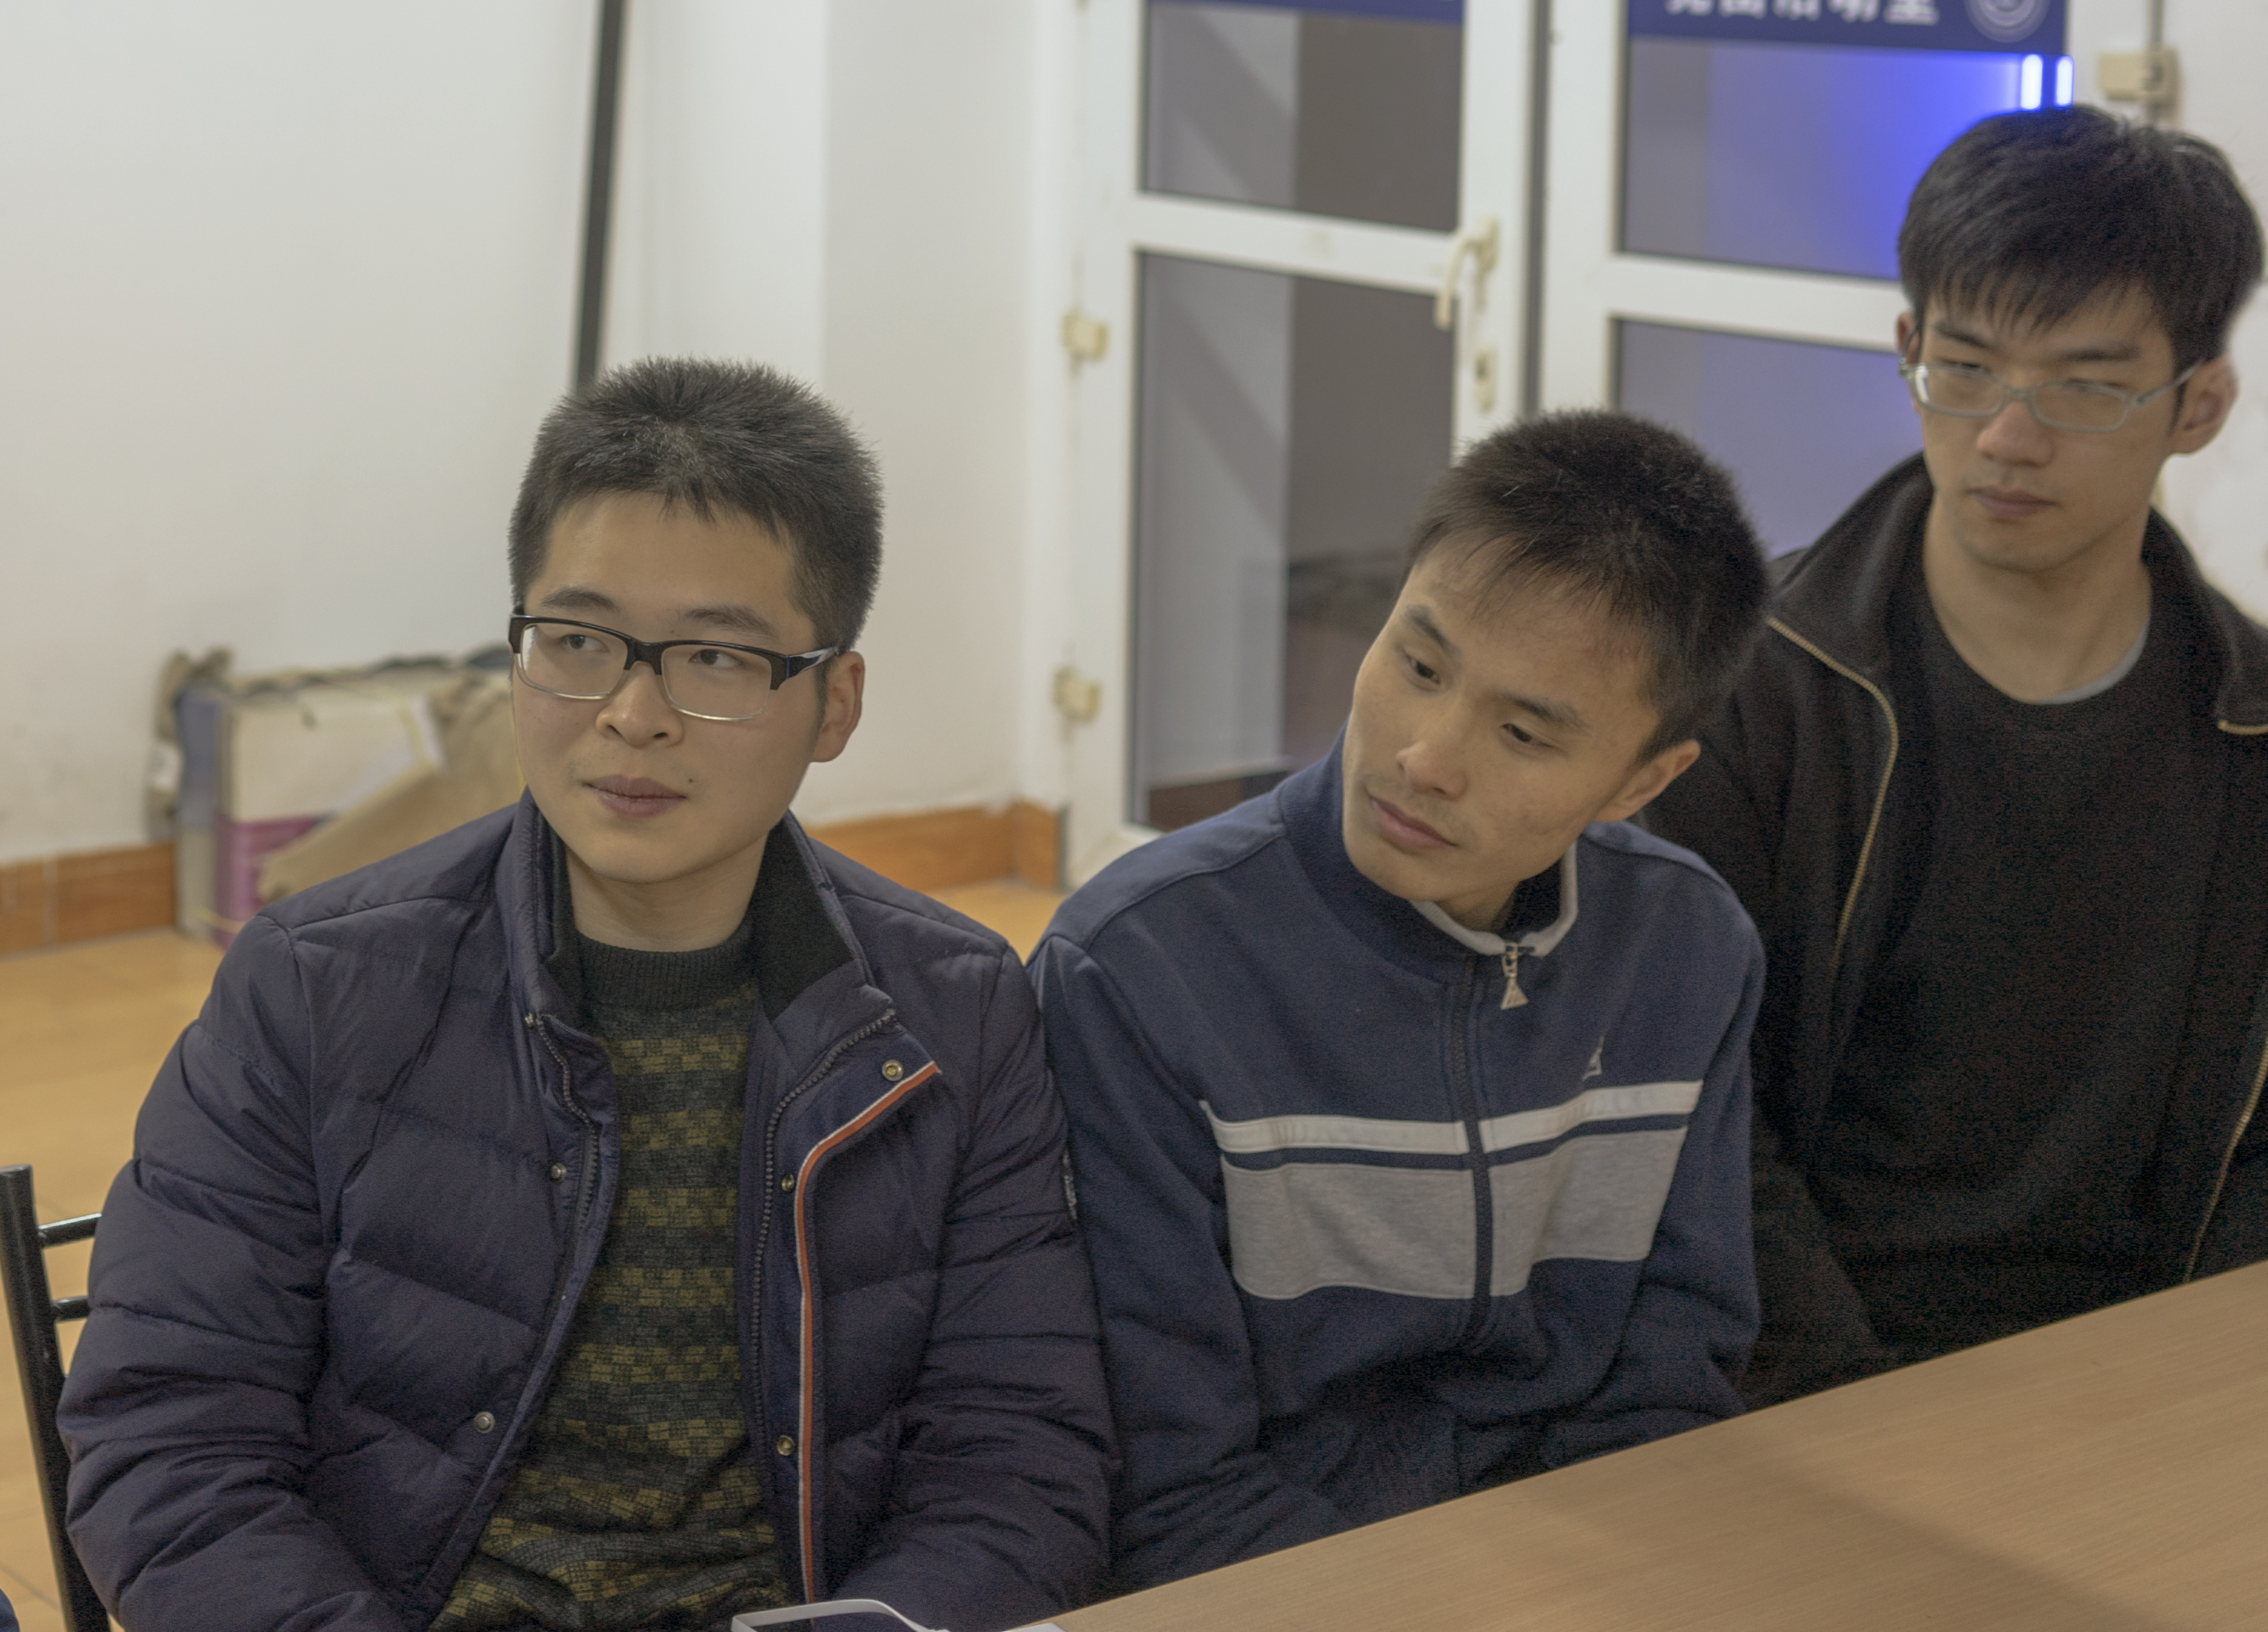
\includegraphics[width=0.8\linewidth,angle=180]{img/sample.jpg}
				\caption{3 greatest people in JI}
				\label{fig-sample}		
			\end{figure}
		\end{example}
	\end{minipage}
	\hfill
	\begin{minipage}{0.5\linewidth}
		\samplecommand{usepackage}\{graphicx\}\\
		\samplebegin{figure}[htbp]\\
		\phantom{\qquad}\samplecommand{centering}\\
		\phantom{\qquad}\samplecommand{includegraphics}[width=0.8\\
		\samplecommand{linewidth},angle=180]\{lena.jpg\}\\
		\phantom{\qquad}\samplecommand{caption}\{3 greatest people in JI\}\\
		\phantom{\qquad}\samplecommand{label}\{fig-sample\}\\
		\sampleend{figure}
	\end{minipage}
\end{frame}

\begin{frame}
	\frametitle{Include multiple graphs}
	Sometimes you need to include a series of graphs, then the \structure{subfigure} package can be used.\\
	\begin{minipage}{0.4\linewidth}
		\begin{example}
			\begin{figure}[htbp]
				\centering
				\subfigure[God Gan]{
					
\includegraphics[width=0.4\linewidth]{img/sample-1.jpg}
					\label{fig-sample-1}
				}
				\subfigure[Master Fu]{
					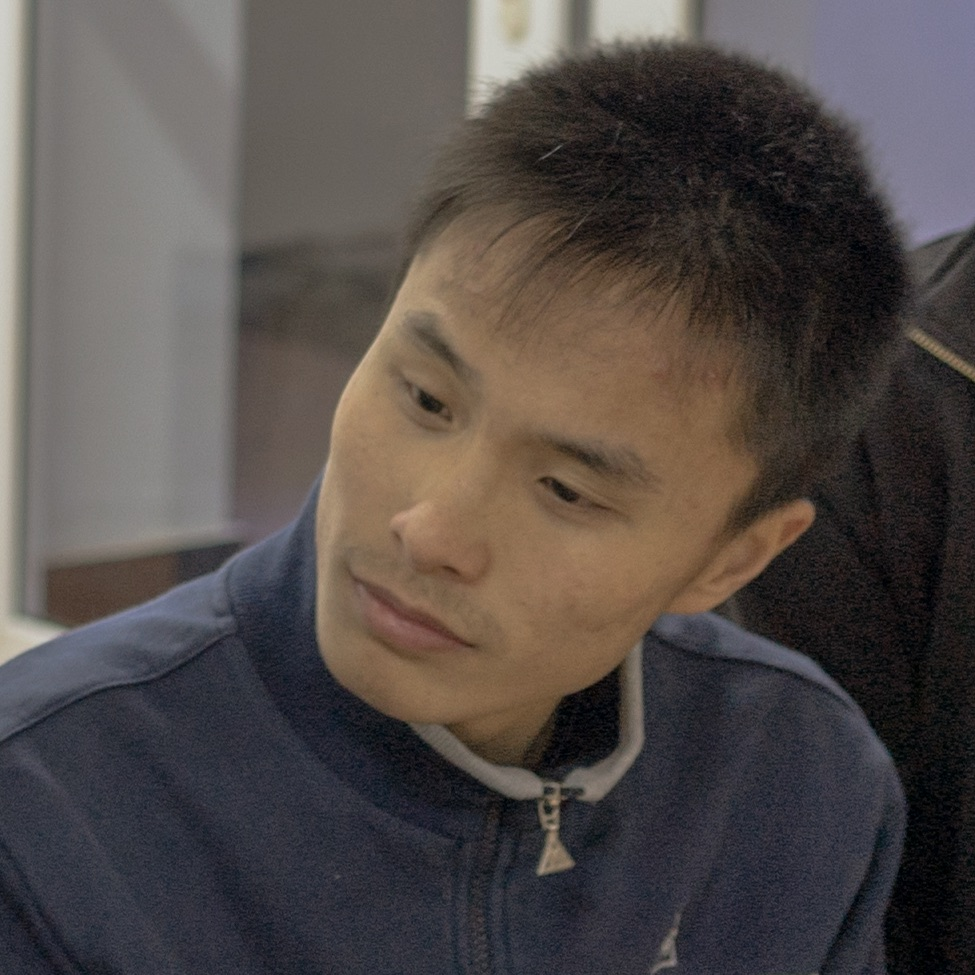
\includegraphics[width=0.4\linewidth]{img/sample-2.jpg}
					\label{fig-sample-2}
				}
				\subfigure[Professor]{
					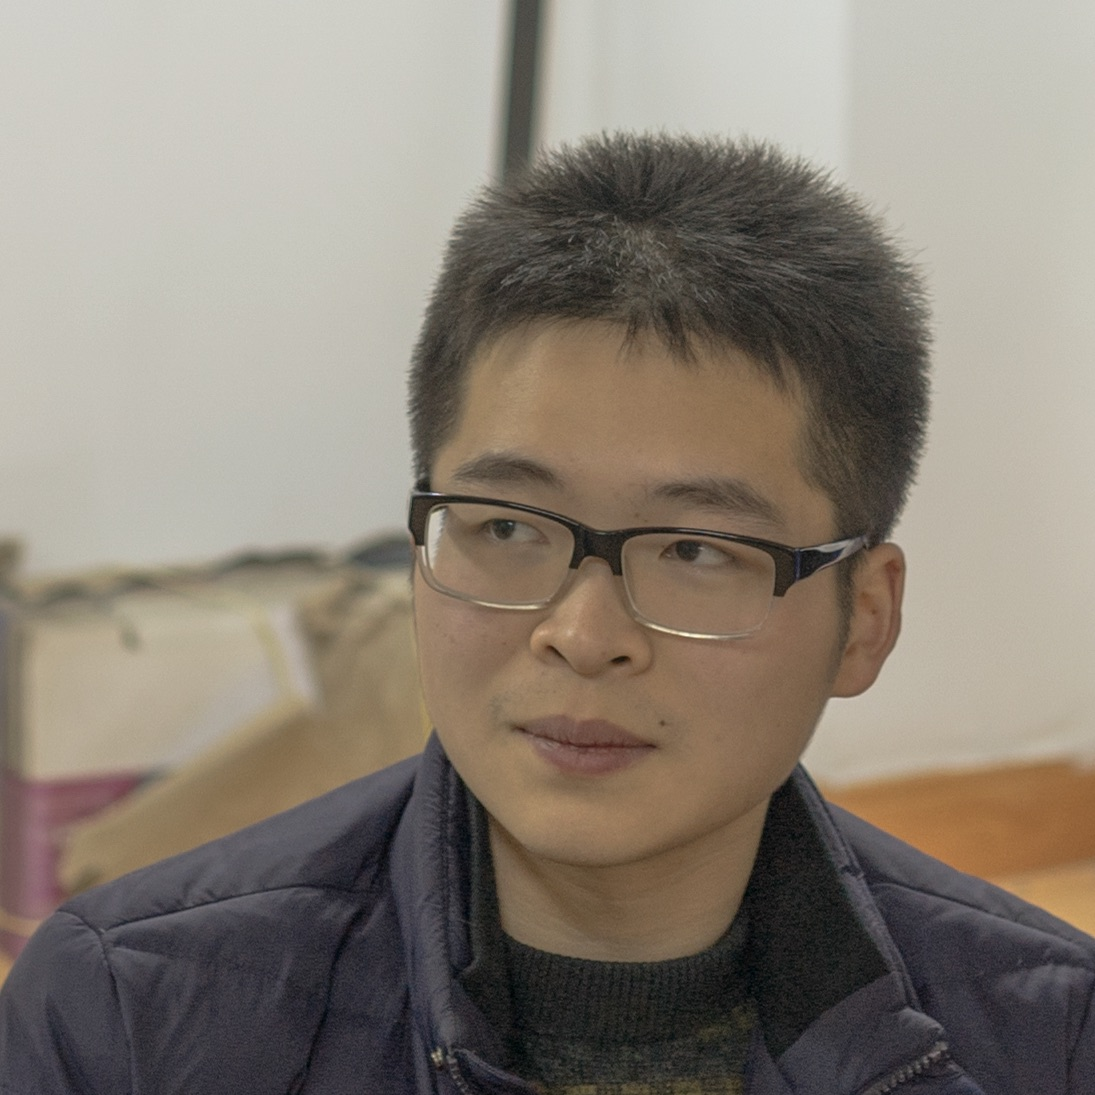
\includegraphics[width=0.4\linewidth]{img/sample-3.jpg}
					\label{fig-sample-3}
				}
				\subfigure[God Hang]{
					
\includegraphics[width=0.4\linewidth]{img/sample-4.jpg}
					\label{fig-sample-4}
				}
			\end{figure}
		\end{example}
	\end{minipage}
	\hfill
		\begin{minipage}{0.55\linewidth}
			\samplecommand{usepackage}\{graphicx\}\\
			\samplecommand{usepackage}\{subfigure\}\\
			\samplebegin{figure}[htbp]\\
			\phantom{\qquad}\samplecommand{centering}\\
			\phantom{\qquad}\samplecommand{subfigure}[God Gan]\{\\
			\phantom{\qquad\qquad}\samplecommand{includegraphics}[width=0.4\\
			\samplecommand{linewidth}]\{sample-1.jpg\}\\
			\phantom{\qquad\qquad}\samplecommand{label}\{fig-sample-1\}\\
			\phantom{\qquad}\}\\
			\phantom{\qquad}\dots(with Master Fu, Professor and God Hang)\\
			\sampleend{figure}
		\end{minipage}
\end{frame}

\subsection{Draw tables}

\begin{frame}
	\frametitle{Draw tables}
	Table is another common element in \LaTeX, for example, there is a simple table like this:
    \begin{example}
        \begin{tabular}{|l|c|r|}
        	\hline
        	Title 1 & Title 2 & Title 3 \\
        	\hline
        	1 & 2 &3 \\
        	\hline
        \end{tabular}
    \end{example}	
	\samplebegin{tabular}\{|l|c|r|\}\\
	\qquad \samplecommand{hline}\\
	\qquad Title 1 \& Title 2 \& Title 3 \samplecommand{\textbackslash} \\
	\qquad \samplecommand{hline}\\
	\qquad 1 \& 2 \& 3 \samplecommand{\textbackslash} \\
	\qquad \samplecommand{hline}\\
	\sampleend{tabular}
\end{frame}

\begin{frame}
	\begin{command}
		\samplebegin{tabular}\{\structure{format}\}\\
		\qquad ...\\
		\sampleend{tabular}
	\end{command}
	\structure{format} can be set as follow
	\begin{itemize}
		\item \structure{|} - represents a vertical separate symbol
		\item \structure{l} - align left in this column
		\item \structure{c} - align center in this column
		\item \structure{r} - align right in this column
	\end{itemize}
	\begin{example}
		\begin{minipage}{0.48\linewidth}
			\centering
			\structure{|l|c|r|}\\[0.5em]
        	\begin{tabular}{|l|c|r|}
        		\hline
        		Title 1 & Title 2 & Title 3 \\
        		\hline
        		1 & 2 &3 \\
        		\hline
        	\end{tabular}
		\end{minipage}
		\begin{minipage}{0.48\linewidth}
			\centering
			\structure{||c|c|c||}\\[0.5em]
        	\begin{tabular}{||c|c|c||}
        		\hline
        		Title 1 & Title 2 & Title 3 \\
        		\hline
        		1 & 2 &3 \\
        		\hline
        	\end{tabular}
		\end{minipage}
    \end{example}	
\end{frame}

\begin{frame}
	\frametitle{Draw tables}
    \begin{example}
        \begin{tabular}{|l|c|r|}
        \hline
        Title 1 & Title 2 & Title 3 \\
        \hline
        1 & 2 &3 \\
        \hline
        \end{tabular}
    \end{example}
    %The example above goes like this:\\
        %$\backslash$begin\{tabular\}\{\mid l\mid c\mid r\mid \} % l represents aligning left; 
        %\\ \qquad \qquad \qquad \qquad \qquad \quad c represents centering; 
        %\\ \qquad \qquad \qquad \qquad \qquad \quad r represents aligning right
        %\\ \qquad \qquad \qquad \qquad \qquad \quad \mid \, means the vertical frame of a column\\
        %$\backslash$hline \quad \% hline means to draw a horizontal line for all columns\\
        %Title 1\&Title 2\&Title 3  \%\& is used to divide contents of different columns\\
        %$\backslash$hline\\
        %1 \& 2 \&3 \\
        %$\backslash$hline\\
        %$\backslash$end\{tabular\}
\end{frame}

\begin{frame}
   \frametitle{Something more about tabular}
   $\backslash$multirow \\
   $\backslash$multicolumn \\
   $\backslash$cline{} \\
\end{frame}

\begin{frame}
	\frametitle{Table environment}
    \begin{definition}
    A \structure{table} environment is used to arrange the place of a tabular
		{\color{red}\textbackslash begin\{table(*)\}[htbp]}\\
		\quad ...\\
		{\color{red}\textbackslash end\{table(*)\}}\\
	\end{definition}
    \text{[h]} means inserting the tabular to the current place.
    \\\text{[t]} means inserting the tabular to the top of the page.
    \\\text{[b]} means inserting the tabular to the bottom of the page.
    \\\text{[p]} means inserting the tabular to another new page, which is common in dealing with big table.
\end{frame}
\begin{frame}
	\frametitle{Insert a graph}
    
\end{frame}

\subsection{Draw graphs}

\begin{frame}

\end{frame}
